\documentclass[twoside,twocolumn, 16pt]{article}

\usepackage{blindtext} % Package to generate dummy text throughout this template 
\usepackage{esvect}
\usepackage[sc]{mathpazo} % Use the Palatino font
\usepackage[T1]{fontenc} % Use 8-bit encoding that has 256 glyphs
\linespread{1.05} % Line spacing - Palatino needs more space between lines
\usepackage{microtype} % Slightly tweak font spacing for aesthetics
\usepackage[utf8]{inputenc}
\usepackage[francais]{babel} % Language hyphenation and typographical rules
\usepackage[T1]{fontenc}
\usepackage{systeme}
\usepackage[hmarginratio=1:1,top=32mm,columnsep=20pt]{geometry} % Document margins
\usepackage[hang, small,labelfont=bf,up,textfont=it,up]{caption} % Custom captions under/above floats in tables or figures
\usepackage{booktabs} % Horizontal rules in tables
\usepackage{csquotes}
\usepackage{graphicx}
\usepackage{caption}
\usepackage{subcaption}
\usepackage{amsmath}
\usepackage{listings}
\usepackage{hyperref}

\newcommand{\icol}[1]{% inline column vector
  \left(\begin{smallmatrix}#1\end{smallmatrix}\right)%
}

\newcommand{\irow}[1]{% inline row vector
  \begin{smallmatrix}(#1)\end{smallmatrix}%
}


\usepackage{lettrine} % The lettrine is the first enlarged letter at the beginning of the text

\usepackage{enumitem} % Customized lists
\setlist[itemize]{noitemsep} % Make itemize lists more compact

\usepackage{abstract} % Allows abstract customization
\renewcommand{\abstractnamefont}{\normalfont\bfseries} % Set the "Abstract" text to bold
\renewcommand{\abstracttextfont}{\normalfont\small\itshape} % Set the abstract itself to small italic text

\usepackage{titlesec} % Allows customization of titles
\renewcommand\thesection{\Roman{section}} % Roman numerals for the sections
\renewcommand\thesubsection{\roman{subsection}} % roman numerals for subsections
\titleformat{\section}[block]{\large\scshape\centering}{\thesection.}{1em}{} % Change the look of the section titles
\titleformat{\subsection}[block]{\large}{\thesubsection.}{1em}{} % Change the look of the section titles

\usepackage{fancyhdr} % Headers and footers
\pagestyle{fancy} % All pages have headers and footers
\fancyhead{} % Blank out the default header
\fancyfoot{} % Blank out the default footer
\fancyhead[C]{Rapport PST $\bullet$ 3GM S2 2017$\bullet$ V.M et R.M} % Custom header text
\fancyfoot[RO,LE]{\thepage} % Custom footer text

\usepackage{titling} % Customizing the title section

\usepackage{hyperref} % For hyperlinks in the PDF

%----------------------------------------------------------------------------------------
%	TITLE SECTION
%----------------------------------------------------------------------------------------

\setlength{\droptitle}{-4\baselineskip} % Move the title up

\pretitle{\begin{center}\Huge\bfseries} % Article title formatting
\posttitle{\end{center}} % Article title closing formatting
\title{Rapport de Projet Scientifique et Technique : fabrication d'un bras robotique de pelleteuse.} % Article title
\author{%
\textsc{Victor Mazoyer \& Robin Menelot} \\[1ex] % Your name
%\textsc{Cyprien Ponçon}\thanks{Corresponding author} \\[1ex] % Second author's name
\normalsize INSA de Lyon \quad Génie Mécanique \\ % Your institution
%\normalsize \href{mailto:john@smith.com}{john@smith.com} % Your email address
%\and  Uncomment if 2 authors are required, duplicate these 4 lines if more
%\textsc{Jane Smith}\thanks{Corresponding author} \\[1ex] % Second author's name
%\normalsize University of Utah \\ % Second author's institution
%\normalsize \href{mailto:jane@smith.com}{jane@smith.com} % Second author's email address
}
\date{} % Leave empty to omit a date
\renewcommand{\maketitlehookd}{%
\begin{abstract}
\noindent Ce rapport présente le Project Scientifique et Techinique que nous avons mené à bien lors de notre second semestre de troisième année au sein du département Génie Mécanique à l'INSA de Lyon. Vous pourrez trouver dans ce rapport la synthèse de notre travail, les méthodes et nos résultats. Nous souhaitons remercier notre tuteur Nans Biboulet pour son soutient, nos coéquipiers qui travaillaient sur des projets similaires et avec qui nous avons su maintenir des relations d'entre-aide. 
\end{abstract}
}

%----------------------------------------------------------------------------------------

\begin{document}

% Print the title
\maketitle

%----------------------------------------------------------------------------------------
%	ARTICLE CONTENTS
%----------------------------------------------------------------------------------------

\section{Introduction}

\lettrine[nindent=0em,lines=3]{L}'objectif est de réaliser un bras de pelleteuse en utilisant un kit de Lego Mindstorms EV3. 
Le kit nous permet de réaliser rapidement des prototypes fonctionnels avec des composants interchangeables.  Nous avions déjà utilisé ce kit pendant la semaine d'intégration de GM et en P2i mécatronique. Cependant nous ne pilotions pas les moteurs/capteurs avec les même outils.

Pour la partie programmation l'objectif est de piloter entièrement le bras à travers un réseau sans fil. Et pour cela il a fallu utiliser et paramètrer un environnement de programmation avec lequel nous n'étions pas familier. Ce projet permet donc d'apprendre à utiliser le terminal Linux, la création d'architecture Réseau sous Python et enfin de gérer les moteurs du Kit Lego.

\subsection{Cahier des charges}
\begin{displayquote}
Voici les instructions que nous avions avant de commencer notre projet : \\
\texttt{Réaliser en lego ev3 une cabine d'engin de chantier type pelleteuse. Commander à travers un réseau sans l les mouvements de l'engin: rotation horizontale, bras, godet. Vous commanderez l'engin en utilisant les capteurs de votre smartphone, un peu comme une manette de Wii, (ou à défaut d'un raspberry équipé d'une board de capteurs).}
\end{displayquote}
%------------------------------------------------

\section{Programmation}
Contrairement à ce qu’il peut paraître, la grosse majorité de notre projet était en réalité de la programmation. Entre l’apprentissage des différents outils, la familiarisation du nouvel environnement informatique et l’écriture du code, notre temps de travail s’est concentré sur la partie numérique du projet. Les choix d’outils liées à notre projet se sont révélés être largement utilisés à travers le monde, et donc on avait accès à de nombreuses aides et ressources sur internet.
\subsection{Architecture}
\subsubsection{Composants du système}
Notre système se compose en quatres parties plus ou moins indépendantes : l’ordinateur, le Raspberry Pi, la brique Lego, les moteurs. Chaques composants joue un rôle particulier et déterminant dans le système. Il nous était imposé d’utiliser chaque composants. \\
\indent \textsc{L'ordinateur} était un élément principal lors de notre travail, en effet, celui-ci nous permettait d’écrire nos programmes, écrire les programmes sur les autres composants via une connection SSH, faire nos recherche et piloter notre bras robotique. On a fait le choix d’utiliser Linux, de naviguer dans nos fichiers et d’écrire nos programmes grâce au Terminal et à l’éditeur de texte Vim. \\
\indent \textsc{Le Raspberry Pi} \footnote{On le référencera par 'RasPi' dans la suite du rapport}, est une carte électronique (de la taille d’une grosse carte bleu), qui se comporte comme un ordinateur. Dotée de port HDMI, USB, d’un émetteur/receveur WIFI, d’un accéléromètre piézoélectrique et bien d’autre encore, nous a servi comme serveur et de relais entre les autres composants, en plus d’être une manette tridimensionnelle pour notre robot. \\ 
\indent \textsc{La brique Lego}, est le relais entre les informations numériques et les sorties mécaniques des moteurs. La briques à pour rôle de convertir les instructions codées en mouvement physique des moteurs constituants notre robot.
\vspace{-1cm}
\subsubsection{Interactions des parties}
Afin de transformer chaque composant indépendant en un système entier il faut les faire communiquer. Au vu de nos connaissances en informatique, on a opté pour une système de communication impliquant des \textsc{sockets}, et donc un système serveur/client.
\begin{center}
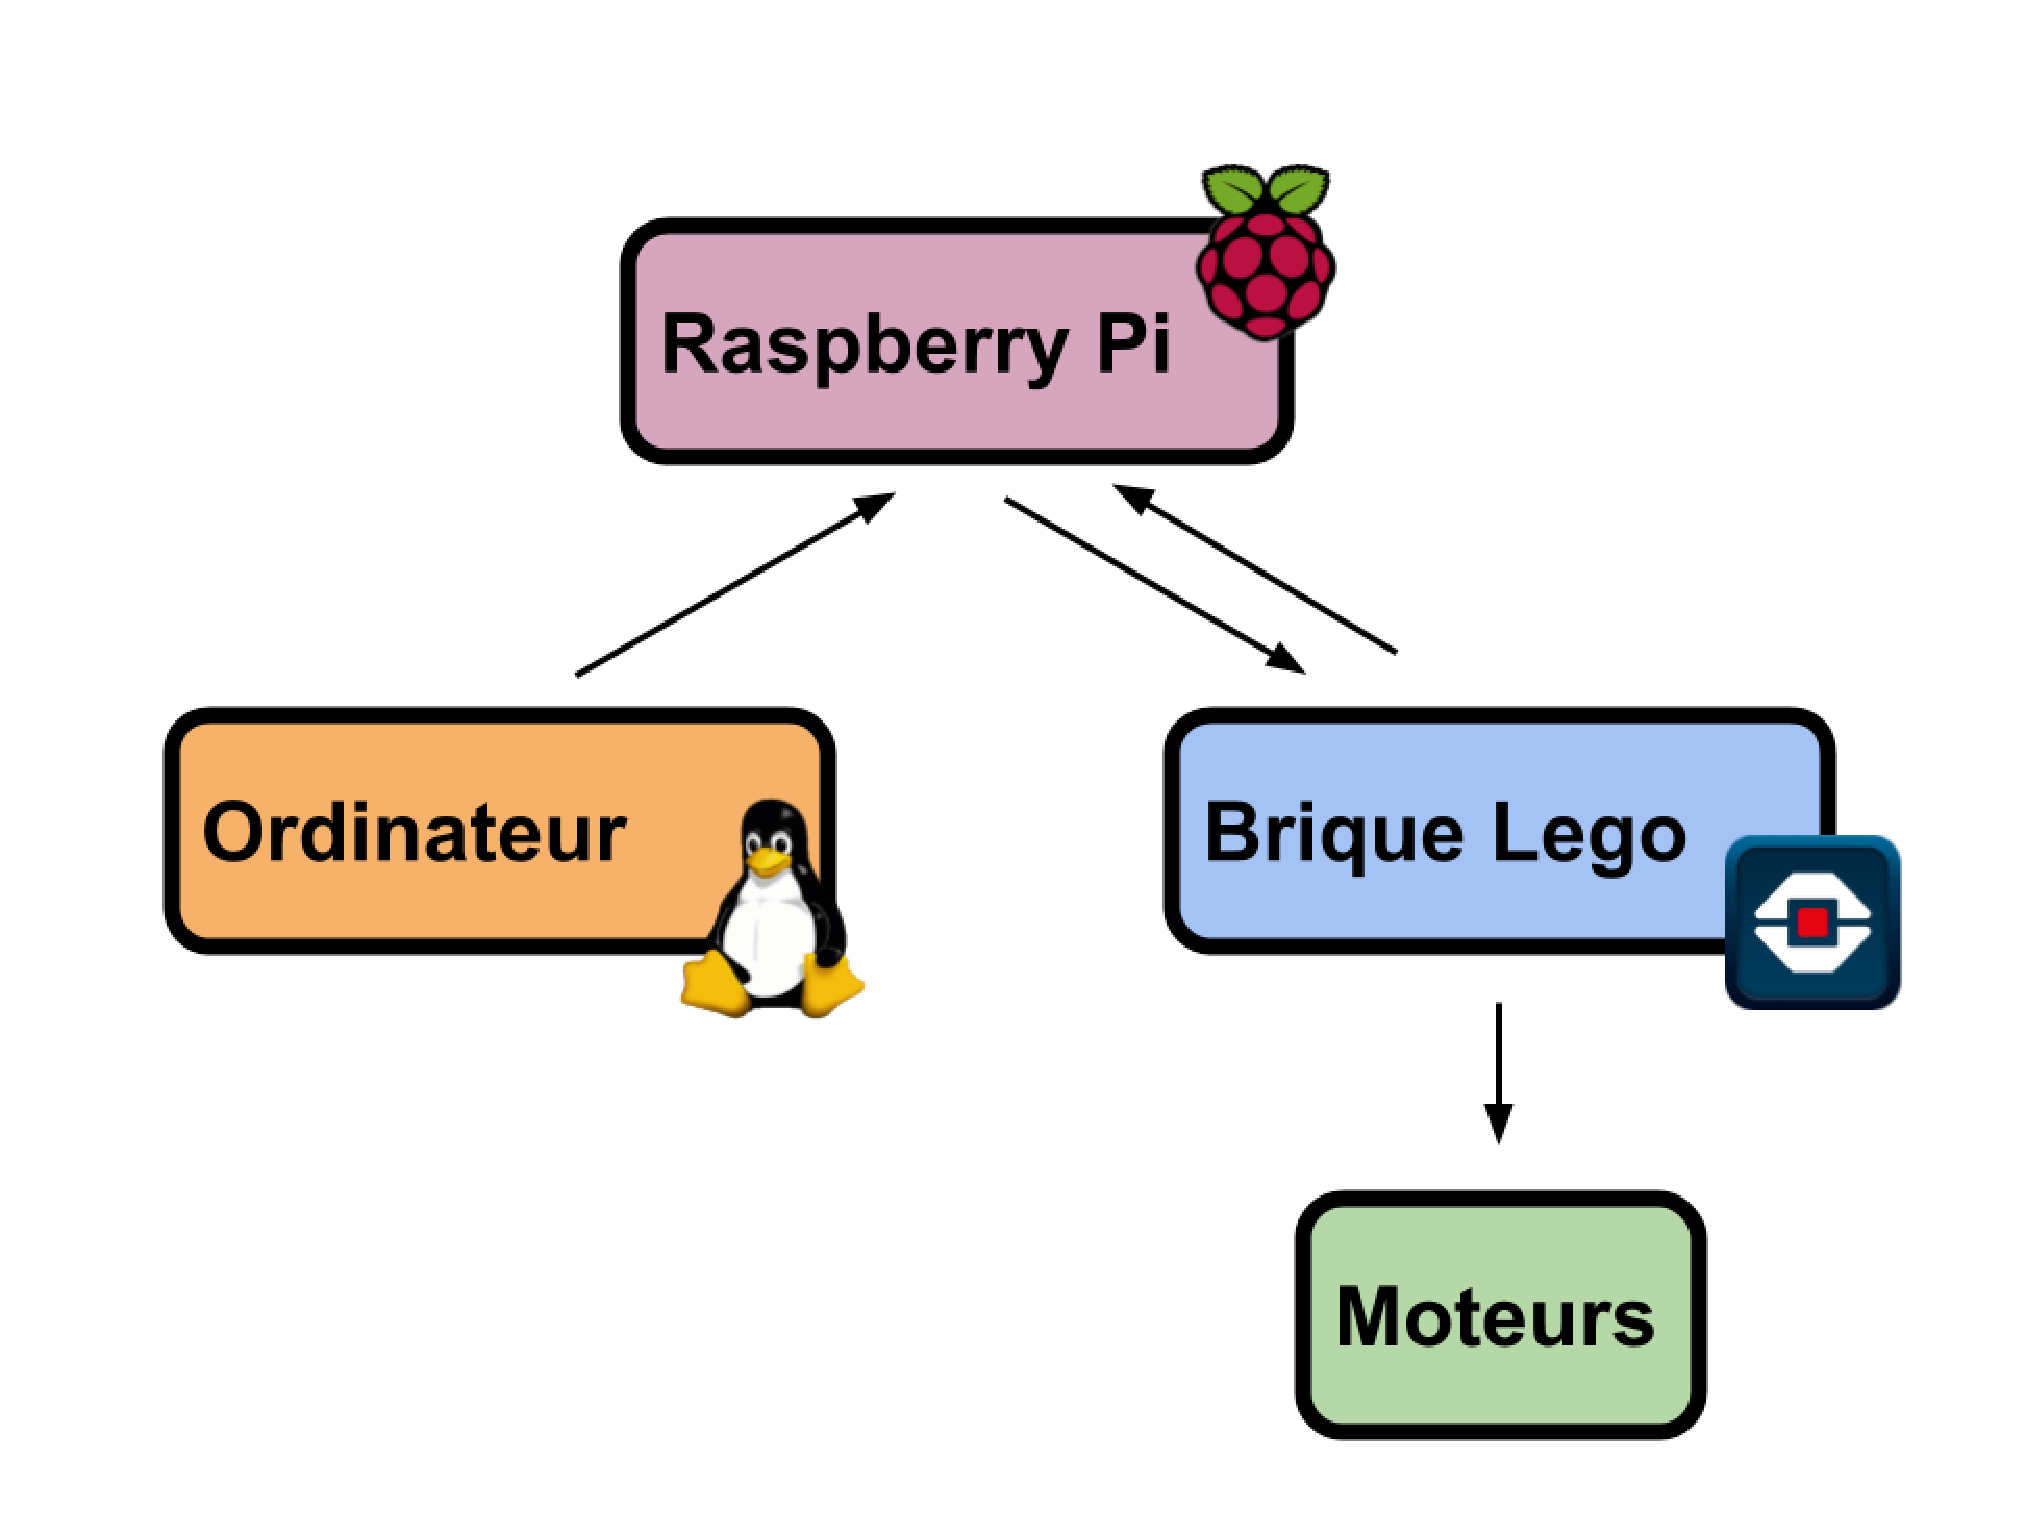
\includegraphics [scale = 0.21] {architecture.eps}
\begin{figure}[!h]
\caption{Diagramme des communications entre les composants}
\end{figure}
\end{center}	
\vspace{-1cm}
\paragraph{} \indent La figure 1 synthétise le fonctionnement des communications entre nos différents composants. On peut voir que le RasPi est un élèment central au protocol, agissant en tant que serveur il devient le relais de chaque transit d'information. On remarque aussi que toutes connections représentées sur le diagramme sont dans la réalité des communications wifi locales, sauf la brique, qui est connectée aux moteurs par des cables élèctroniques. Notre sytème présente deux fonctionalités avec deux protocoles légèrement différents. \\
\indent La première, comme indiquée dans le cahiers des charges, une télécomande tridimensionnelle qui pilote les différents moteurs en fonction de ses déplacements dans l'espace (façon manette de Wii). Ce protocole ne requiert par l'ordinateur; un \textsc{thread} de communication python est ouvert entre le RasPi et la brique, on récupère les accélérations des capteurs piézoélectriques du RasPi avant des les analyser et les envoyer à la brique par wifi. Le fonctionement du système sera expliqué plus loin dans le rapport. \\ 
\indent La seconde, un désir de notre part (notamment à cause de la faible précision de la prmière façon de fonctionner), était de pouvoir controler les moteurs grâce au clavier de l'ordinateur. On a simplement rajouté l'ordinateur à la communication, le RasPi communique donc avec deux clients simultanement. Il est d'autant plus important d'établir un protocole de communication rigoureu afin d'établir les règles et l'ordre des informations échangées entre les composants.

%------------------------------------------------

\subsection{Code}
Cette section a pour but d'expliquer les outils principaux utilisés lors de la programmation. Il faut savoir que le language utlisé pour la programmation de notre système est le \textsc{python}. Ce choix nous était d'une part imposé, mais s'est révélé judicieux de part la grande quantité de docuementation et le \textsc{libraries} disponible sur internet.\\
\subsubsection{Terminal Linux et SSH}
Notre environement de travail informatique peut se résumer au Terminal Linux et son éditeur de texte Vim. L'utilisation simple des commandes \textsc{cd, ls, makedir} ainsi que \textsc{vim} et \textsc{python3} nous on rapidement permis de prendre en main les outils pour débuter notre programmation. \\
\indent La connection SSH était aussi une partie importante, puisque c'est grace à celle-ci que nous pouvions sans effort écrire des programmes sur les différents composant. Avec une simple ligne de code dans le Terminal on pouvait commencer à programmer sur les appareils.
\subsubsection{Socket}
Les \textsc{sockets} existent dans différents languages informatique, dans notre cas la \textsc{python}. Elles sont au centre des systèmes de communication, nous ne nous sommes pas penché vers les détails de leurs fonctionnements. En revanche, on savait qu'il fallait choisir judicieusement le serveur et les clients. Nous avons choisi le RasPi pour trois raisons : c'est un appreil à la puissance de calcul rapide contrairement à la brique Lego; il est présent dans les deux protocole de communication, c'était donc plus simple pour nous; finalement, il est au centre des transits d'information, c'est donc une minimisation du nombre de transfert d'information, et donc une optimisation. 

\subsubsection{Capteurs piézoélectrique}

En utilisant les capteurs du RasPi et les libraries XLoBorg, on pu simplement extraire les accélérations (en multiple de $\vec{g}$, l'accélération terrestre) dans les directions $\icol{x\\y\\z}$ du repère du RasPi. 
\begin{center}
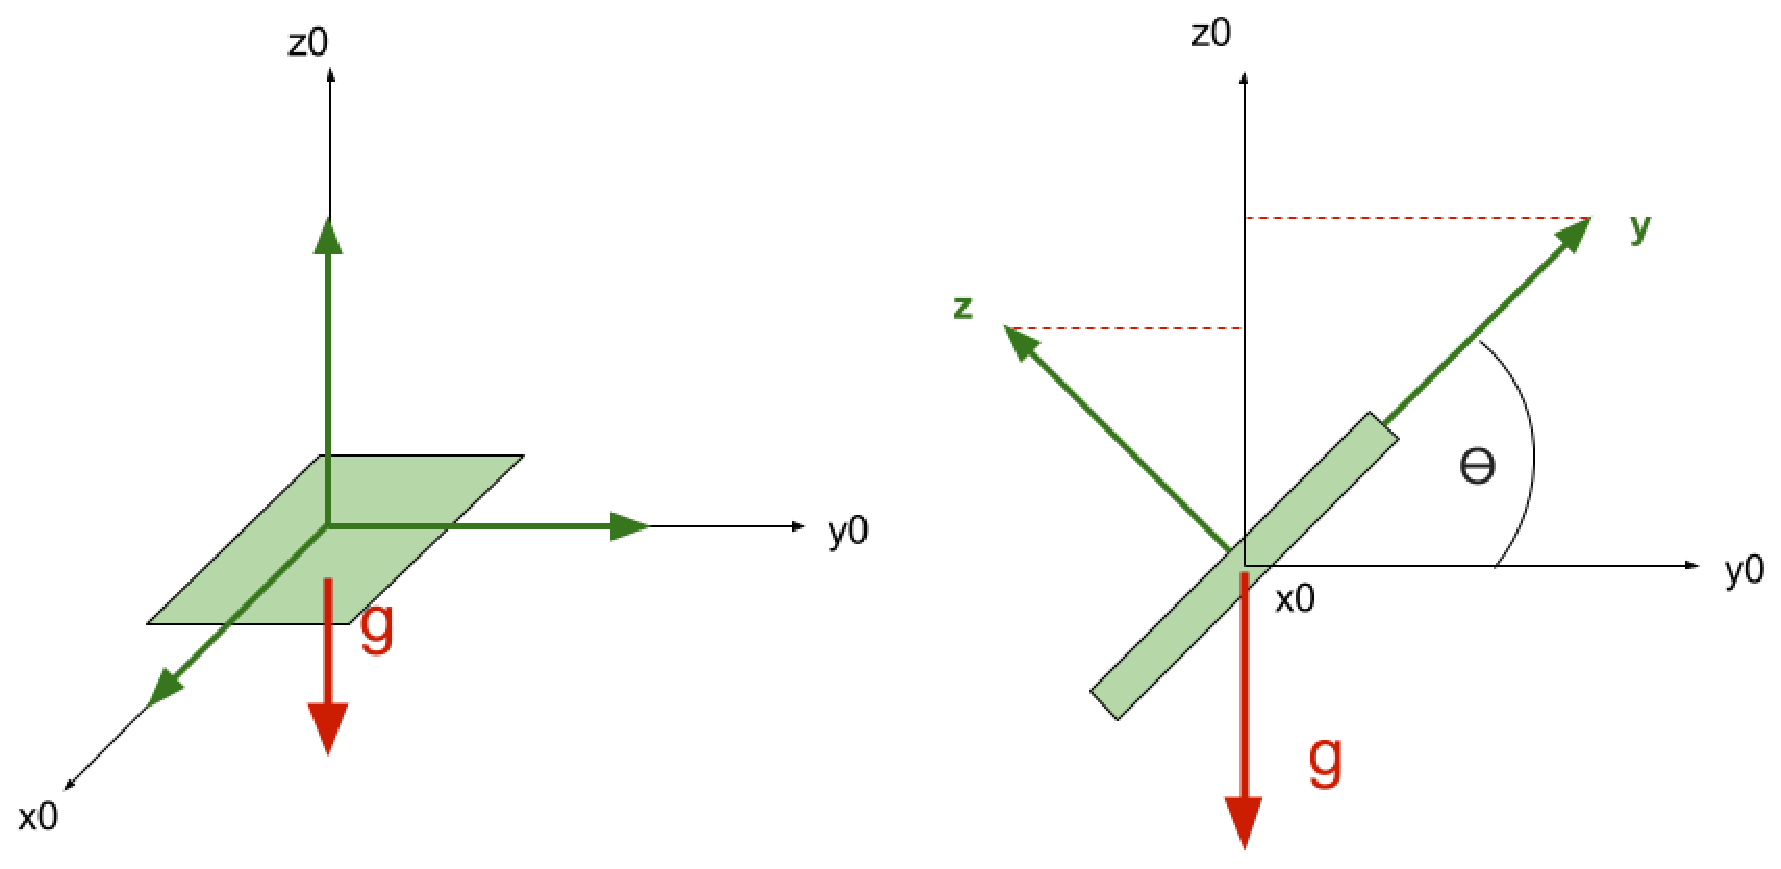
\includegraphics [scale = 0.23] {acc.eps}
\begin{figure}[!h]
\caption{Schema qui reprérente le repère galiléen, le repère du RasPi et l'accélration terreste.}
\end{figure}
\end{center}
Lorsque le RasPi est à plat les valeurs retournées sont $\icol{0\\0\\-1}$ car c'est la projection de $\vec{g}$ sur le repère du RasPi. Maintenant, si on incline le RasPi d'un angle $\theta$ selon $x_0$, les projections deviennent :
\begin{center}
$\icol{x\\y\\z} \cdot \vec{g} =$ \systeme*{ 0 , - g \sin{\theta},  - g \cos{\theta} } \\
\end{center}
\indent On peut donc voir que la direction dans laquelle l'accélération est nulle, est l'axe de rotation du RasPi. Tout ceci est bien joli, mais ne fonctionnent que pour les axes $x$ et $y$ car il est impossible d'exploiter $\vec{g}$ afin d'avoir  $\vec{z} \cdot \vec{g} = 0$ et des valeurs non nulles dans les deux autres directions. Ceci veut dire qu'on a seulement deux degrés de liberté, donc qu'on ne peut controler que deux moteurs indépendement. \\
\indent On a pensé à une solution afin de contourner le problème, mais elle semblait au-dessus de nos compétences. Il s'agit d'établir un changement de base du repère associé au RasPi pour le transformé en "pyramide inversé", cela aurais la conséquence de parvenir à des projection de $\vec{g}$ non nulles dans toutes les directions. 

\subsubsection{Getch}
\textsc{getch} nous a servis à la lecture en continu des touches du clavier. Pour controler le robot à l'aide des flèches du clavier on devait mettre en place un système de \textsc{Key Listener} non-bloquant et continu. Les libraries Getch on remplis cette fonction.

\subsubsection{Library EV3}
Les lignes de codes présente sur la brique Lego sont majoritairement des instructions pour les moteurs. Ces lignes de code font appel à des fonctions disponibles dans des libraries en open-source sur internet. Voici un exmple d'une ligne de code qui fait appelà une fonction \textsc{ev3} : \\
\vspace{-0.5cm}
\begin{lstlisting}
mB.run_timed(time_sp=600, 
speed_sp=600)
\end{lstlisting}
Ici cette ligne de code ordonne au moteur B de tourner pendant 600 ms à vitesse 600 (échelle de puissance : [0 , 1400]).

%------------------------------------------------

\section{Mécanique}
%A statement requiring citation \cite{Figueredo:2009dg}.

Intro chapitre mécanique \\
construciton par essai et echec \\
bricolage \\
on a fait ça comme mais ça aurais pu être différent \\
introduire les legos 

\subsection{Cinématique du bras}
plagia sur bras de pellteuse \\
on avait que 3 moteurs \\
image de scheme cinématique +commentaire \\

\begin{center}
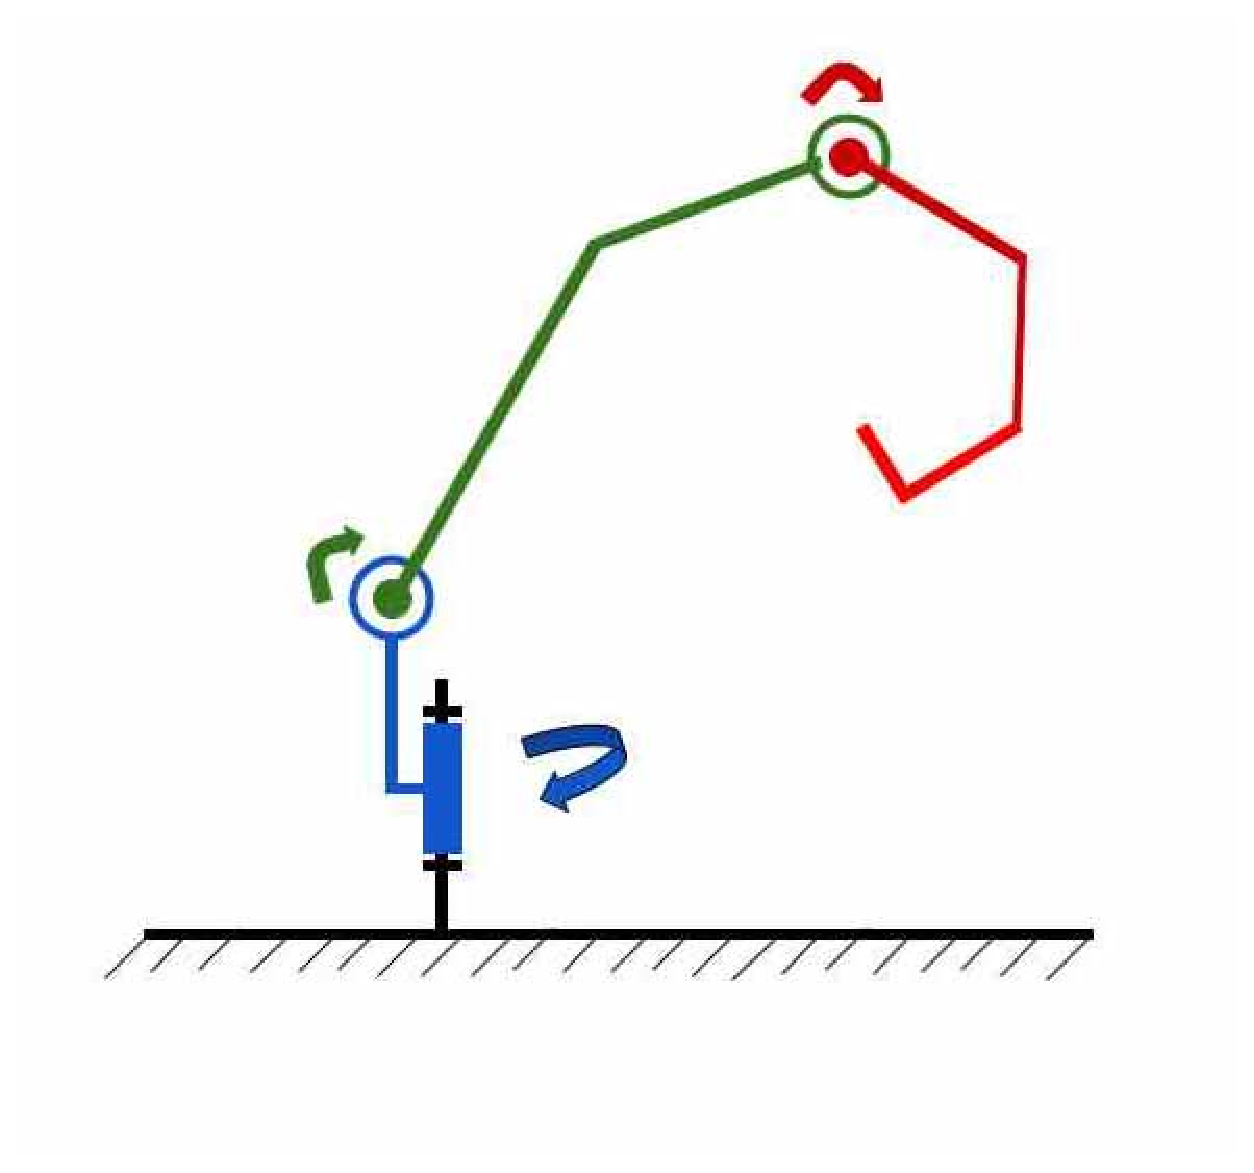
\includegraphics[scale = 0.3]{cin.eps}
\begin{figure}[!h]
\caption{Schema cinématique du bras robotique.}
\end{figure}
\end{center}

\subsection{Construction}
parler vite fait des lego \\
parler des problème : elastique + vis sans fin (avec photo de la vis)

\subsubsection{Prototype}
finir par photo du prototype final
et parler de ce qu'on a réussi à faire concretement

%----------------------------------------------------------------------------------------
%	REFERENCE LIST
%----------------------------------------------------------------------------------------

\begin{thebibliography}{99} % Bibliography - this is intentionally simple in this template

\bibitem{ev3pythonlibrary}
EV3 PYTHON. Learn EV3 Python [en ligne]. Disponible sur : \\\url{https://sites.google.com/site/ev3python/} (22/03/17)

\bibitem{xloborg}
PiBorg. Robotics add on boards for use with your Raspberry Pi [en ligne]. Disponible sur : \\
\url{https://www.piborg.org/xloborg} (19/05/17)
 
 \bibitem{pstBiboulet}
 N. Biboulet. Démarage PST Lego [PDF] 2017. 7 pages.
\end{thebibliography}

%----------------------------------------------------------------------------------------
\newpage
\section{Annexes}
\subsection{Programmes sur ordinateur}
\subsubsection{clientPCv1.py}
\begin{lstlisting}
import socket
import time
from Getch import Getch,whatKeyIsPressed

if __name__ == '__main__':
	
	s = socket.socket()
	host = '192.168.42.1'
	port = 8087
	s.connect((host,port))
	
	while True:
		time.sleep(0.1)
		key = whatKeyIsPressed()
		s.send(key.encode())
		print(key)
		if key == 'q':
			s.close()
			break
}
\end{lstlisting}

\subsubsection{Getch.py}

\begin{lstlisting}
class Getch:
	def __init__(self):
		import tty, sys

	def __call__(self):
		import sys, tty, termios
		fd = sys.stdin.fileno()
		old_settings = termios.tcgetattr(fd)
		try:
			tty.setraw(sys.stdin.fileno())
			ch = sys.stdin.read(1)
		finally:
			termios.tcsetattr(fd, termios.TCSADRAIN, old_settings)
		return ch

def whatKeyIsPressed () :
	while True:
		init = Getch()()
		if init == 'q':
			return 'q'
			break
		if init == 'z':
			return 'z'
		if init == 's':
			return 's'
		elif init == '\033':
			Getch()()
			key = Getch()()
			if key=='A':
				return 'up'
			if key=='B':
				return 'down'
			if key=='C':
				return 'right'
			if key=='D':
				return 'left'
\end{lstlisting}



\end{document}